As we have seen, Alastria is a Spanish blockchain consortium, in which multiple companies and organizations are collaborating in different Github repositories\footnote{https://github.com/alastria}, promoting the implementation of a new digital identity model known as \acrlong{ssi}. In Alastria this implementation is called Alastria ID. Its mission is to reach all sectors and contribute to the creation of an innovation ecosystem that is as diverse as possible. \\

\begin{figure}[h]
    \centering
    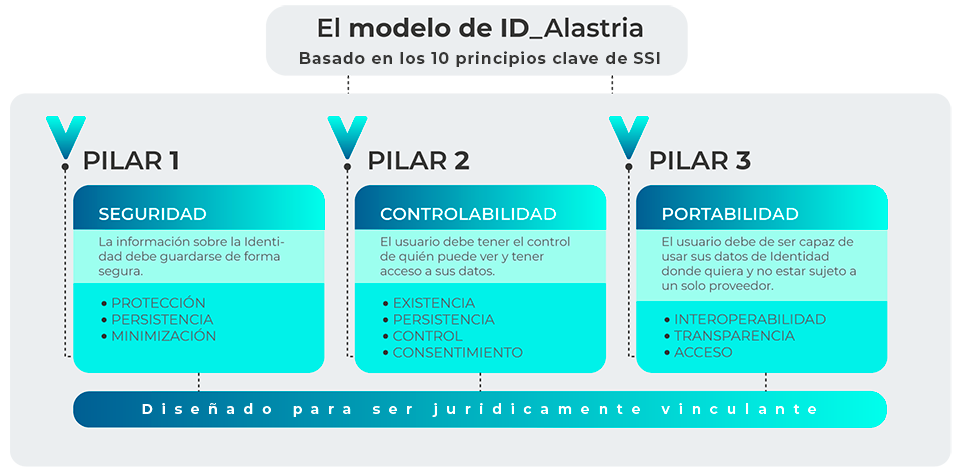
\includegraphics[width=1.0\textwidth]{images/Alastria ID/pilares_alastria.png}
    \caption{Alastria ID model}
    \label{fig:pilares_alastria}
\end{figure}

As the figure \ref{fig:pilares_alastria} obtained from the Alastria main website\footnote{https://alastria.io/en/id-alastria/} represents, the Alastria ID model is based in the 10 key principles of the \acrshort{ssi}. It is designed to be legally binding, and its three fundamental pillars are:
\begin{itemize}
    \item \textbf{Security}: identity information must be kept secure. This means protection, persistence and minimization.
    \item \textbf{Controllability}: the user must have control of who can see and have access to their data. This means existence, persistence, control and consent.
    \item \textbf{Portability}: the user must be able to use their data wherever they want and not be subject to a single provider. This means interoperability, transparency and access.
\end{itemize}

